\documentclass{article}
\usepackage[utf8]{inputenc}
\usepackage{graphicx}

\usepackage{enumerate}
\begin{document}
\section{Online naručivanje i dostava hrane i pića}
Online naručivanje i dostava hrane i pića je slučaj upotrebe gde mušterija definiše svoju narudžbinu, radnici je prave, a dostavljači isporučuju. U naručivaju učestvuju: mušterija, radnik i dostavljač.
\\
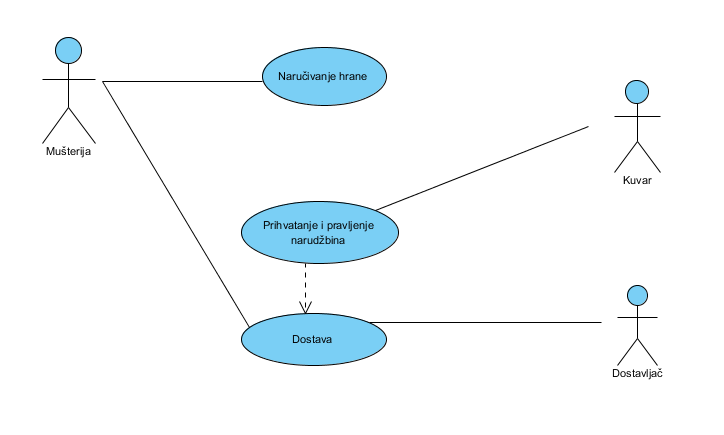
\includegraphics[width=\linewidth]{narucivanjeIdostava.png}


\subsection{\textbf{Use Case}: Pravljenje narudžbine}
\textbf{Akter:} Mušterija\\
\textbf{Ulaz:} Nema\\
\textbf{Izlaz:} Definisana narudžbina\\
\textbf{Preduslovi:} Restoran prima narudžbine\\
\textbf{Postuslov:} Uspešno napravljena narudžbina je poslata restoranu\\
\textbf{Glavni tok:}
\begin{enumerate}
\item Ukoliko mušterija nema nalog na sistemu, vrši registraciju i dobija korisničko ime i lozinku od sistema
\item Mušterija unosi korisničko ime i lozinku
\item Mušterija se prijavljuje na sistem
\item Mušterija vrši odabir hrane i pića
\item Mušterija ostavlja podatke o adresi za dostavu
\item Mušerija potvrdjuje narudžbinu, koja se dalje prosledjuje na sistem
\end{enumerate}
\textbf{Alternativni tok:} \\
        3.1. Prijavljivanje nije uspešno, mušterija se vraća na korak 2\\


\subsection{\textbf{Use Case}: Prihvatanje i pravljenje narudžbina}
\textbf{Akter:} Radnik, Dostavljač\\
\textbf{Ulaz:} Spisak narudžbina\\
\textbf{Izlaz:} Napravljene narudžbine\\
\textbf{Preduslovi:} Radnik se uspešno ulogovao na sistem i spiskovi narudžbina su uspešno stigli do njega\\
\textbf{Postuslov:}  Napravljene narudžbine su spremne za dostavu\\
\textbf{Glavni tok:}
\begin{enumerate}
\item Radnik uzima spiskove narudžbina
\item Za svaku narudžbinu iz spiska pravi se porcija, po redosledu vremena naručivanja
\item Po završetku pravljenja obroka, radnik obaveštava Dostavljača da je porudžbina spremna za dostavu 
\end{enumerate}
\textbf{Alternativni tok:}\\
       2.1. Ukoliko  fale sastojci za neku od narudžbina, prelazi se na sedeću narudžbinu dok sastojci ne stignu\\
       
       
\subsection{\textbf{Use Case}: Dostava i prihvatanje dostave}
\textbf{Akter:} Dostavljač, Mušterija\\
\textbf{Ulaz:} Pripremljena narudžbina\\
\textbf{Izlaz:} Izvršena dostava\\
\textbf{Preduslovi:} Mušterija je ispravno definisala adresu\\
\textbf{Postuslov:}  Izvršena dostava je plaćena\\
\textbf{Glavni tok:}
\begin{enumerate}
\item Dostavljač odnosi porudžbina na adresu definisanu na narudžbini
\item Mušterija prihvata porudžbinu i proverava da li je sve u redu sa sadržajem
\item Mušterija plaća dostavu
\end{enumerate}
\textbf{Alternativni tok:}\\
       2.1 Ukoliko nije sve u redu sa sadržajem, pravi se nova narudžbna i mušterija čeka novu dostavu, ili mušterija odustaje od narudžbine\\
       2.2 Ukoliko je mušterija odustala, dostavljač vraća hranu u restoran

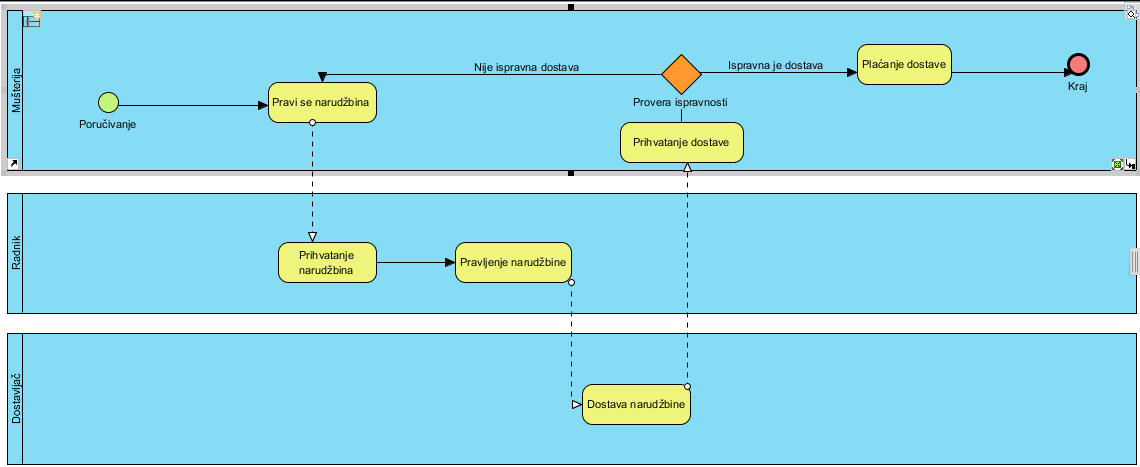
\includegraphics[width=\textwidth]{dostavaBPMN.png}
\end{document}
